% document formatting
\documentclass[10pt]{article}
\usepackage[utf8]{inputenc}
\usepackage[left=1in,right=1in,top=1in,bottom=1in]{geometry}
\usepackage[T1]{fontenc}
\usepackage{xcolor}

% math symbols, etc.
\usepackage{amsmath, amsfonts, amssymb, amsthm}

% lists
\usepackage{enumerate, enumitem}

% images
\usepackage{graphicx} % for images

% code blocks
\usepackage{minted, listings} 

% verbatim greek
\usepackage{alphabeta}

\graphicspath{{./assets/images}}

\newcommand{\solution}{\textbf{Solution:}} 
\newcommand{\example}{\textbf{Example:}}

\title{COM SCI M151B Week 10}

\author{Aidan Jan}
\date{\today}

\begin{document}
\maketitle
\section*{System}
\begin{itemize}
    \item There is more to a modern computer than just the processor and memory.
    \item Other components are generally referred to as Input/Outputs, or I/Os.
\end{itemize}
\subsection*{Example}
\begin{center}
    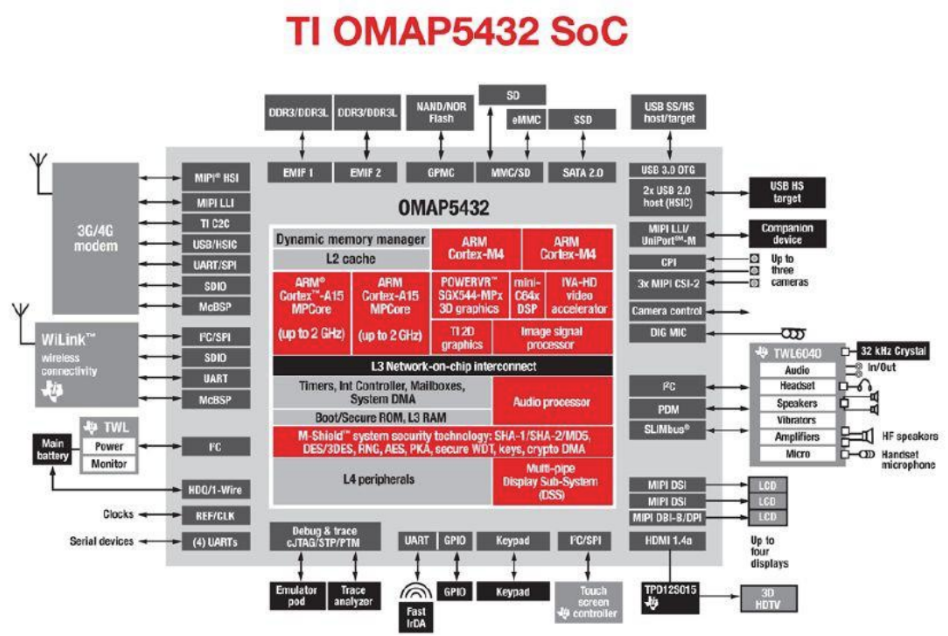
\includegraphics[scale=0.6]{W10_1.png}
\end{center}
\subsection*{I/O}
\begin{itemize}
    \item Various I/Os depending on the class of the computer (e.g., PC, Server, Mobile, Embedded)
    \item Broad categories:
    \begin{itemize}
        \item Secondary/Tertiary storage (flash, disk, tape)
        \item Network (Ethernet, WiFi, Bluetooth, LTE)
        \item Human-machine interfaces (keyboard, mouse, touchscreen, graphics, audio, video, neural, ...)
        \item Printers (line, laser, inkjet, photo, 3D, ...)
        \item Sensors (process control, GPS, heart rate, ...)
        \item Actuators (valves, robots, car brakes, ...)
    \end{itemize}
\end{itemize}
\subsection*{Structure}
\begin{center}
    \includegraphics*[scale=0.6]{W10_2.png}
\end{center}
\subsection*{How to Read/Write from/to IO}
\begin{itemize}
    \item Directly using Channels/Registers
    \begin{itemize}
        \item Dedicate a specific set of registers to read/write (e.g., mainly in microcontrollers).
        \item Having a dedicated channel (e.g., writing to a specific pin).
    \end{itemize}
    \item Memory-Mapped I/O
    \begin{itemize}
        \item Map a reserved part of the memory addresses to the I/O.
        \item Reading and writing to I/Os become loads and stores to specific addresses.
        \item Typically "uncached" memory addresses (using page tables).
        \item Virtual address?
    \end{itemize}
\end{itemize}

\subsection*{How to Communicate}
\begin{itemize}
    \item Different technologies and protocols (various needs and available technologies through decades)
    \begin{itemize}
        \item Time multiplexed Shared and slow (very slow!) \textrightarrow~PCI, IDE
        \item Shared but fast(er) \textrightarrow~Ethernet, SATA
        \item Dedicated channel \textrightarrow~PCIE
        \item Handshaking \textit{asynchronous} through arbiter, initiator, and target or fixed timing protocol.
    \end{itemize}
\end{itemize}

\subsection*{DMA}
\begin{itemize}
    \item MMIO is slow, so why not talking directly to the memory?
    \begin{itemize}
        \item Use a separate unit called direct memory access (DMA)
    \end{itemize}
    \item DMA engines offload CPU by autonomously transferring data between I/O device and main memory.  CPU can be notified when DMA is done with transaction
    \item DMA programmed through memory-mapped registers
    \item Some systems use dedicated processors inside DMA engines.
    \item Often, many separate DMA engines in modern systems.
\end{itemize}

\subsection*{Modern I/O}
\begin{center}
    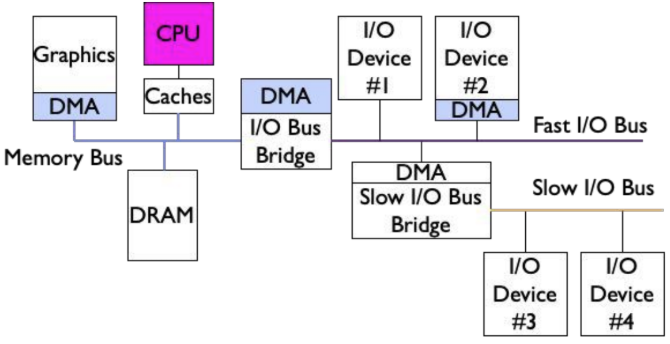
\includegraphics[scale=0.7]{W10_3.png}
\end{center}

\subsection*{Network on Chip (NoC)}
\begin{itemize}
    \item Different technologies and protocols
    \begin{itemize}
        \item Multiple cores
        \item Memory hierarchy (on-chip and off-chip)
        \item GPU
        \item Accelerators
        \item I/O
    \end{itemize}
\end{itemize}
\begin{center}
    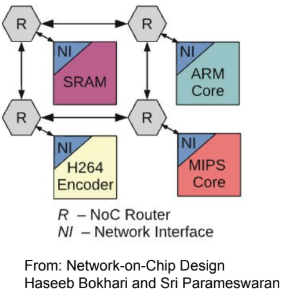
\includegraphics[scale=0.9]{W10_4.png}\\
    \includegraphics*[scale=0.6]{W10_5.png}
\end{center}
\subsection*{Challenges}
\begin{itemize}
    \item Many challenges:
    \begin{itemize}
        \item Performance optimization
        \item Scalability
        \item Energy efficiency
        \item Security
        \item Integration with emerging computing paradigms
    \end{itemize}
    \item Main design ingredients:
    \begin{itemize}
        \item Topology, protocols, routing logic, router design, etc.
        \item Bandwidth and latency \textrightarrow~different technologies
    \end{itemize}
\end{itemize}
\subsection*{Interacting with Core}
\begin{itemize}
    \item Communication between I/O and CPU requires a timing mechanism.
    \item Interrupt vs. Polling
\end{itemize}
\subsubsection*{Interrupt}
\begin{itemize}
    \item If an event occurs, then call a service routine (a function stored in the reserved space of the main memory) to handle it.
    \item Pro: no CPU overhead until the event happens
    \item Con: can happen at unexpected and unwanted times
    \item Con: large context-switch overhead
\end{itemize}
\subsubsection*{Polling}
\begin{itemize}
    \item Checking the event with some predetermined frequency.
    \item Con: CPU overhead
    \item Con: Difficult to implement
    \item Pro: Can be fully scheduled
\end{itemize}
\subsubsection*{Hybrid}
\begin{itemize}
    \item Interrupt on first event, use polling for some time, switch back to interrupt after sufficient time.
\end{itemize}
\subsection*{Exception, Traps, Interrupts}
\begin{itemize}
    \item Exception refers to an unusual condition occurring at run time associated with an instruction in the current thread/process.
    \item Trap refers to the synchronous transfer of control to a handler caused by an exceptional condition occurring within a thread (i.e., similar to jumping to a routine).
    \item Interrupt refers to an external event that occurs asynchronously to the current thread.
    \begin{itemize}
        \item To service an interrupt, an interrupt exception occurs, and the CPU subsequently experiences a trap.
    \end{itemize}   
\end{itemize}
\subsubsection*{Examples:}
Branch Mispredictions causes an exception
\begin{itemize}
    \item To handle this exception, the CPU has to recover by flushing ROB, RS, etc.
    \item A successful recovery requires maintaining all the necessary states for each instruction (e.g., RAT table), so we call this a precise exception.
    \item 
\end{itemize}
I/O events causes interrupts
\begin{itemize}
    \item To handle this interrupt, the CPU has to trap, and send the control to interrupt handler.
    \item When to trap depends on the interrupt's priority
\end{itemize}
OS System Call causes a trap.
\begin{itemize}
    \item To invoke a service from the OS, the CPU has to execute a trap to transform the control into a handler.
    \item Trap usually has a parameter indicating which service it needs.  Handler uses a table to jump to the corresponding subroutine to handle the requested service.
\end{itemize}
Other examples:
\begin{itemize}
    \item Unknown instruction \textrightarrow~exception (issues a trap to handle)
    \item Hardware failure \textrightarrow~exception/trap
    \item Overflow
    \item etc.
\end{itemize}
\begin{center}
    \includegraphics*[width=\textwidth]{W10_6.png}
\end{center}


\end{document}